% !TEX root = ../../../main.tex
% 来源：中学数学实验教材·第三册（高中数学）
% 章节：函数及其图象 / 一次函数（线性函数）
% 原始文件：4.tex，行 1487-1519
% 类型：tikz
% ---
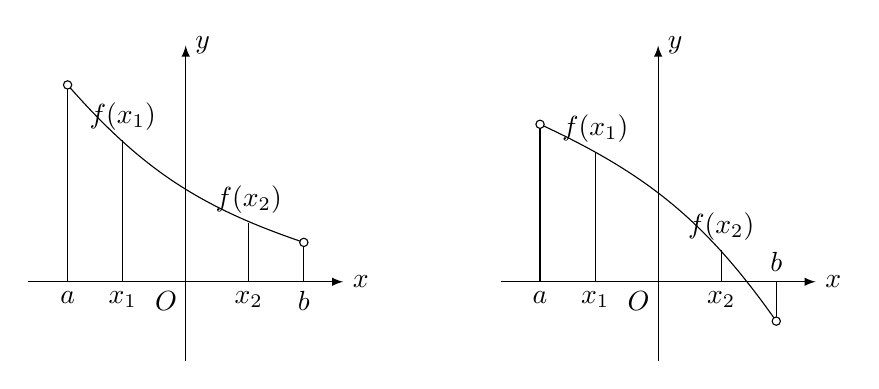
\begin{tikzpicture}[>=latex]
\begin{scope}
    \draw[->](-2,0)--(2,0)node[right]{$x$};  
\draw[->](0,-1)--(0,3)node[right]{$y$};
\node at (-.25,-.25){$O$};
\draw (-1.5,2.5) to [bend left=-15] (1.5,.5);
\draw (-1.5,2.5)--(-1.5,0)node[below]{$a$};
\draw (1.5,.5)--(1.5,0)node[below]{$b$};

\draw (-.8,1.8)node[above]{$f(x_1)$}--(-.8,0)node[below]{$x_1$};
\draw (.8,.75)node[above]{$f(x_2)$}--(.8,0)node[below]{$x_2$};




\draw (-1.5,2.5) [fill=white]circle(1.5pt) ;
\draw (1.5,.5) [fill=white]circle(1.5pt) ;
\end{scope}
\begin{scope}[xshift=6cm]
    \draw[->](-2,0)--(2,0)node[right]{$x$};  
    \draw[->](0,-1)--(0,3)node[right]{$y$};
    \node at (-.25,-.25){$O$};
    \draw (-1.5,2) to [bend left=15] (1.5,-.5);
    \draw (-1.5,2)--(-1.5,0)node[below]{$a$};
    \draw (1.5,-.5)--(1.5,0)node[above]{$b$};
    \draw (-.8,1.65)node[above]{$f(x_1)$}--(-.8,0)node[below]{$x_1$};
    \draw (.8,.4)node[above]{$f(x_2)$}--(.8,0)node[below]{$x_2$};
    

    \draw (-1.5,2) [fill=white]circle(1.5pt) ;
    \draw (1.5,-.5) [fill=white]circle(1.5pt) ;  
\end{scope}    
\end{tikzpicture} 
